\section{Templates}

\subsection{Variadic Templates}

\begin{frame}[fragile]{Variadic Templates}
    \begin{cpp}
template <typename T>
inline void read(T &x) {
  int c = getchar(), f = 0; x = 0;
  while (!isdigit(c)) {
    f |= c == '-';
    c = getchar();
  }
  while (isdigit(c)) {
    x = x * 10 + c - '0';
    c = getchar();
  }
  if (f) x = -x;
}
template <typename T, typename... Args>
inline void read(T &x, Args &...args) {
  read(x); read(args...);
}
    \end{cpp}
\end{frame}

\begin{frame}[fragile]{Variadic Templates}
    \begin{cpp}
int a; long b; unsigned c; short d;
read(a, b, c, d);
    \end{cpp}
    \pause
    The compiler will generate:
    \begin{cpp}
void read(int &, long &, unsigned &, short &);
void read(long &, unsigned &, short &);
void read(unsigned &, short &);
void read(short &);
void read(int &);
void read(long &);
void read(unsigned &);
    \end{cpp}
\end{frame}

\begin{frame}[fragile]{Pack Expansion}
    When \ttt{Args \&...args} becomes
    \begin{cpp}
long &a, unsigned &b, short &c
    \end{cpp}
    the expression \ttt{read(args...)} expands to
    \begin{cpp}
read(a, b, c);
    \end{cpp}
    \begin{itemize}
        \item e.g. \ttt{\&args...} expands to \ttt{\&a, \&b, \&c}.
        \item e.g. \bluett{const\_cast}\ttt{<const Args *>(\&args)...} expands to
        \begin{cpp}
const_cast<const T1 *>(&x1), const_cast<const T2 *>(&x2), const_cast<const T3 *>(&x3)
        \end{cpp}
        \item \bluett{sizeof}\ttt{...(args)} is the number of elements in the parameter pack. (NOT `\bluett{sizeof}\ttt{(args)...}'!)
    \end{itemize}
\end{frame}

\subsection{Specialization: Revisit}

\begin{frame}[fragile]{Check whether Two Types are Same}
    \begin{cpp}
template <typename X, typename Y>
struct AreSame {
  static constexpr bool value = false;
};
template <typename X>
struct AreSame<X, X> {
  static constexpr bool value = true;
};

AreSame<int, double>::value // false
AreSame<int, signed>::value // true
    \end{cpp}
\end{frame}

\begin{frame}[fragile]{Check whether a Type is a Pointer}
    \begin{cpp}
template <typename T>
struct IsPointer {
  static constexpr bool value = false;
};
template <typename T>
struct IsPointer<T *> {
  static constexpr bool value = true;
};
    \end{cpp}
\end{frame}

\begin{frame}{\ttt{<type\_traits>}}
    \begin{center}
        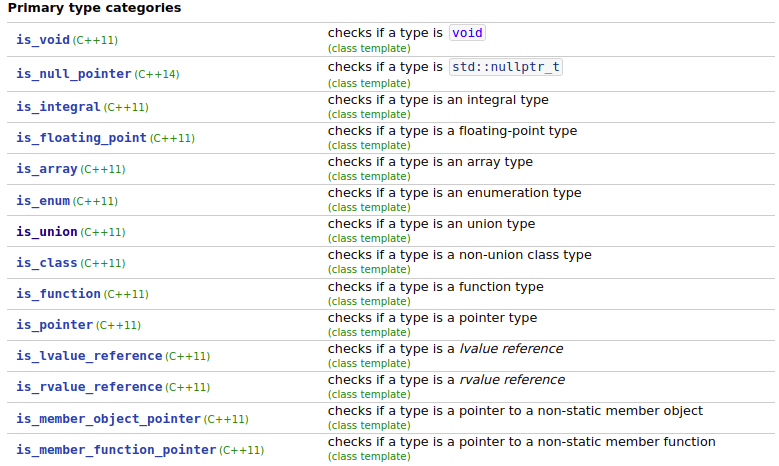
\includegraphics[width = \textwidth]{img/typetraits1.png}
    \end{center}
\end{frame}

\begin{frame}{\ttt{<type\_traits>}}
    \begin{center}
        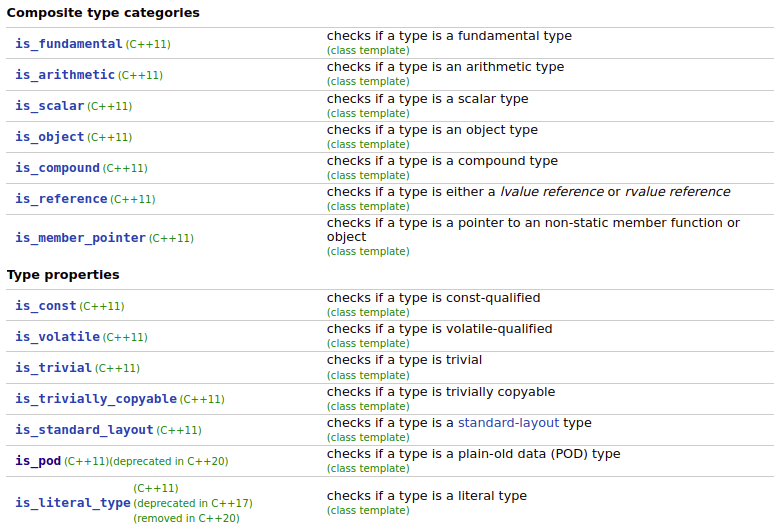
\includegraphics[width = \textwidth]{img/typetraits2.png}
    \end{center}
\end{frame}

\begin{frame}{\ttt{<type\_traits>}}
    \begin{center}
        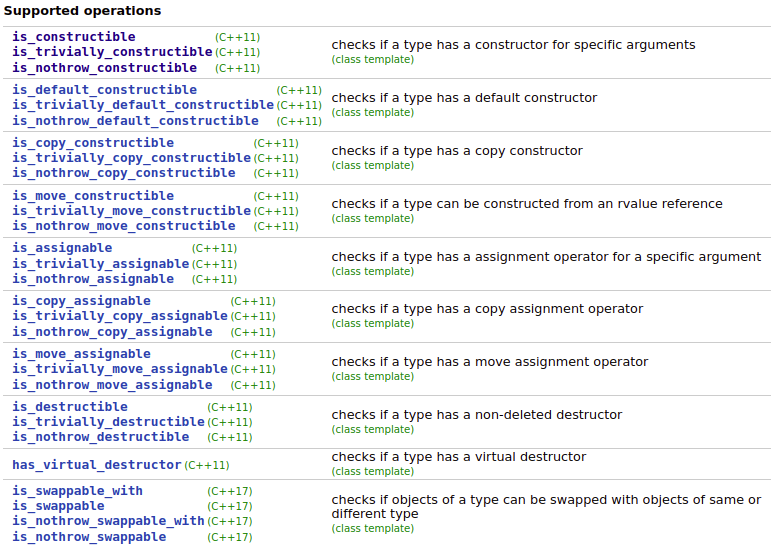
\includegraphics[width = 0.95\textwidth]{img/typetraits3.png}
    \end{center}
\end{frame}

\begin{frame}[fragile]{Examples}
    Raise a compile-error with customized information text when \ttt{Shape} is not an abstract class:
    \begin{cpp}
static_assert(std::is_abstract<Shape>::value,
              "'Shape' must be an abstract class!");
    \end{cpp}
    \pause
    \ttt{std::vector} doesn't allow value-type to be cv-qualified:
    \begin{cpp}
template <typename Tp, typename Alloc>
class vector {
  static_assert(std::is_same<Tp, typename std::remove_cv<Tp>::type>::value, "std::vector must have a non-const, non-volatile value type!");
  // ...
};
    \end{cpp}
\end{frame}

\begin{frame}[fragile]{Examples}
    \begin{cpp}
template <typename Tp, typename Alloc>
class vector {
  static_assert(std::is_same<Tp, typename std::remove_cv<Tp>::type>::value, "std::vector must have a non-const, non-volatile value type!");
  // ...
};
    \end{cpp}
    Why is \typename here?
    \pause
    \begin{itemize}
        \item When \ttt{Tp} is unknown, the compiler does not know what \ttt{std::remove\_cv<Tp>} is.
        \item Is \ttt{std::remove\_cv<Tp>::type} a type or a \bluett{static} data member? You tell the compiler.
    \end{itemize}
\end{frame}

\begin{frame}[fragile]{Examples}
    \begin{cpp}
template <typename T, bool is_const>
class Slist_iterator {
 public:
  using reference = typename std::conditional<is_const, const T &, T &>::type;
  using pointer = typename std::conditional<is_const, const T *, T *>::type;
};
    \end{cpp}
    \pause
    How is \ttt{std::conditional} implemented?
\end{frame}

\begin{frame}[fragile]{Examples}
    \begin{cpp}
template <bool Condition, typename TrueT, typename FalseT>
struct Conditional {
  using type = TrueT;
};
template <typename TrueT, typename FalseT>
struct Conditional<false, TrueT, FalseT> {
  using type = FalseT;
};
    \end{cpp}
\end{frame}

\begin{frame}[fragile]{\ttt{std::distance}}
    \begin{cpp}
template <typename Iterator>
?? distance(Iterator begin, Iterator end);
    \end{cpp}
    What's the return-type?
    \pause
    \begin{cpp}
typename Iterator::difference_type
    \end{cpp}
\end{frame}

\begin{frame}[fragile]{\ttt{std::distance}}
    Is this correct?
    \begin{cpp}
template <typename Iterator>
  typename Iterator::difference_type
    distance(Iterator begin, Iterator end) {
  return end - begin;
}
    \end{cpp}
    \pause
    Yes, but only for \blue{random-access-iterator}s.
\end{frame}

\begin{frame}[fragile]{\ttt{std::distance}}
    Recognize and choose different implementations:
    \begin{itemize}
        \item For \blue{input-iterator}s, increment \ttt{begin} until it reaches \ttt{end} and count the steps.
        \item For \blue{random-access-iterator}s, return \ttt{end - begin}.
    \end{itemize}
    \pause
    Require every iterator to have a type alias member: \ttt{iterator\_category}.
    \begin{itemize}
        \item \ttt{std::vector<T>::iterator\_category} is \ttt{std::random\_access\_iterator\_tag}
        \item \ttt{std::list<T>::iterator\_category} is \ttt{std::bidirectional\_iterator\_tag}
        \item \ttt{std::forward\_list<T>::iterator\_category} is \ttt{std::forward\_iterator\_tag}
    \end{itemize}
\end{frame}

\begin{frame}[fragile]{\ttt{std::distance}}
    \begin{cpp}
template <typename Iterator>
auto distance_impl(Iterator begin, Iterator end,
                   std::input_iterator_tag) {
  // ...
}
template <typename Iterator>
auto distance_impl(Iterator begin, Iterator end,
                   std::random_access_iterator_tag) {
  return end - begin;
}
template <typename Iterator>
inline auto distance(Iterator begin, Iterator end) {
  using category = typename Iterator::iterator_category;
  return distance_impl(begin, end, category{});
}
    \end{cpp}
    \begin{itemize}
        \item ``Compile-time polymorphism''.
    \end{itemize}
\end{frame}

\begin{frame}[fragile]{Traits}
    Wait... What about pointers?
    \begin{itemize}
        \item Pointers are also iterators,
        \item but they do not have a `\ttt{iterator\_category}' member!
    \end{itemize}
    \pause
    \begin{cpp}
template <typename Iterator>
struct Category {
  using type = typename Iterator::iterator_category;
};
template <typename T>
struct Category<T *> {
  using type = std::random_access_iterator_tag;
};
    \end{cpp}
\end{frame}

\begin{frame}[fragile]{Traits}
    \begin{cpp}
template <typename Iterator>
struct Category {
  using type = typename Iterator::iterator_category;
};
template <typename T>
struct Category<T *> {
  using type = std::random_access_iterator_tag;
};
template <typename Iterator>
inline auto distance(Iterator begin, Iterator end) {
  return distance_impl(begin, end,
                    typename Category<Iterator>::type{});
}
    \end{cpp}
\end{frame}

\begin{frame}[fragile]{\ttt{std::iterator\_traits}}
    The standard library has defined \ttt{std::iterator\_traits}:
    \begin{cpp}
template <typename Iterator>
struct iterator_traits {
  using value_type = typename Iterator::value_type;
  using difference_type
      = typename Iterator::difference_type;
  using pointer = typename Iterator::pointer;
  using reference = typename Iterator::reference;
  using iterator_category
      = typename Iterator::iterator_category;
};
    \end{cpp}
\end{frame}

\begin{frame}[fragile]{\ttt{std::iterator\_traits}}
    Specialization of \ttt{std::iterator\_traits} for pointers:
    \begin{cpp}
template <typename T>
struct iterator_traits<T *> {
  using value_type = T;
  using difference_type = std::ptrdiff_t;
  using pointer = T *;
  using reference = T &;
  using iterator_category
      = std::random_access_iterator_tag;
};
    \end{cpp}
\end{frame}

\subsection{SFINAE Examples}

\begin{frame}[fragile]{Test whether a Function Exists}
    SFINAE: Substitution Failure Is Not An Error
    \begin{itemize}
        \item When substitution failure happens, the compiler tries some other solutions instead of reporting an error.
        \pause
        \item If we can transform an error into a substitution failure...
    \end{itemize}
    \pause
    \begin{cpp}
namespace detail {
  template <typename T = Expr,
            typename = decltype(make_sin((T *)nullptr))>
  std::true_type helper(int);
  std::false_type helper(double);
}
constexpr bool make_sin_defined
    = decltype(detail::helper(0))::value;
    \end{cpp}
    \begin{itemize}
        \item That's how things like \ttt{std::is\_copy\_constructible} are implemented.
    \end{itemize}
\end{frame}

\begin{frame}[fragile]{Test whether a Member Function is \ttt{const}}
    \begin{cpp}
namespace detail {
  template <typename T = Point_handle,
            typename = decltype(((const T *)nullptr)->get_x())>
  std::true_type helper(int);
  std::false_type helper(double);
}
constexpr bool get_x_is_const
    = decltype(detail::helper(0))::value;
static_assert(get_x_is_const, "Why don't you define get_x as a const member function?");
    \end{cpp}
\end{frame}

\begin{frame}[fragile]{\ttt{std::enable\_if}}
    Enable a function to be called according to a given condition:
    \begin{cpp}
template <typename T>
inline auto read(T &x) // Only allow T to be integral type
    -> typename std::enable_if<std::is_integral<T>::value,
                               void>::type {
  // ...
}
    \end{cpp}
\end{frame}

\begin{frame}[fragile]{\ttt{std::enable\_if}}
    Allow conversion from \ttt{iterator} to \ttt{const\_iterator}:
    \begin{cpp}
template <typename T, bool is_const>
class Slist_iterator {
 public:
  template <typename Other,
            typename = typename std::enable_if<
                std::is_same<Slist_iterator<T, false>,
                             Other>::value
                && is_const>::type>
  Slist_iterator(const Other &oi);
};
    \end{cpp}
\end{frame}

\subsection{Template Metaprogramming}

\begin{frame}[fragile]{Compile-time Factorial}
    Compile-time factorial:
    \begin{cpp}
template <unsigned N>
struct Factorial {
  static constexpr unsigned value
      = N * Factorial<N - 1>::value;
};
template <>
struct Factorial<0> {
  static constexpr unsigned value = 1;
};
    \end{cpp}
    You may use it like this:
    \begin{cpp}
std::cout << Factorial<5>::value;  // prints 120
std::cout << Factorial<10>::value; // prints 3628800
    \end{cpp}
    The results are calculated during compile-time!
\end{frame}

\begin{frame}{What can it Accomplish?}
    Examples:
    \begin{itemize}
        \item Ensuring dimensional unit correctness
        \item Optimizing matrix operations
        \item Generating custom design pattern implementations
        \item Designing ``domain-specific embedded languages'' (DSEL).
    \end{itemize}
\end{frame}

\begin{frame}[fragile]{A Simple Example: Dimensions}
    From \textit{C++ Template Metaprogramming} Chapter 3:
    \begin{cpp}
#include "dimensions.hpp"
#include <iostream>
int main() {
    quantity<double, mass> m(3.0);
    quantity<double, force> f(6.0);
    quantity<double, acceleration> a(2.0);
    quantity<double, force> f2 = m * a;
    std::cout << f2.value() << std::endl;
    std::cout << (m * a == f) << std::endl;
    f += -m * a + f;
    std::cout << f.value() << std::endl;

    // This should cause a compile-error.
    std::cout << (m + f).value() << std::endl;
    return 0;
}
    \end{cpp}
\end{frame}